%!TEX root = ../Main.tex
\begin{figure}
  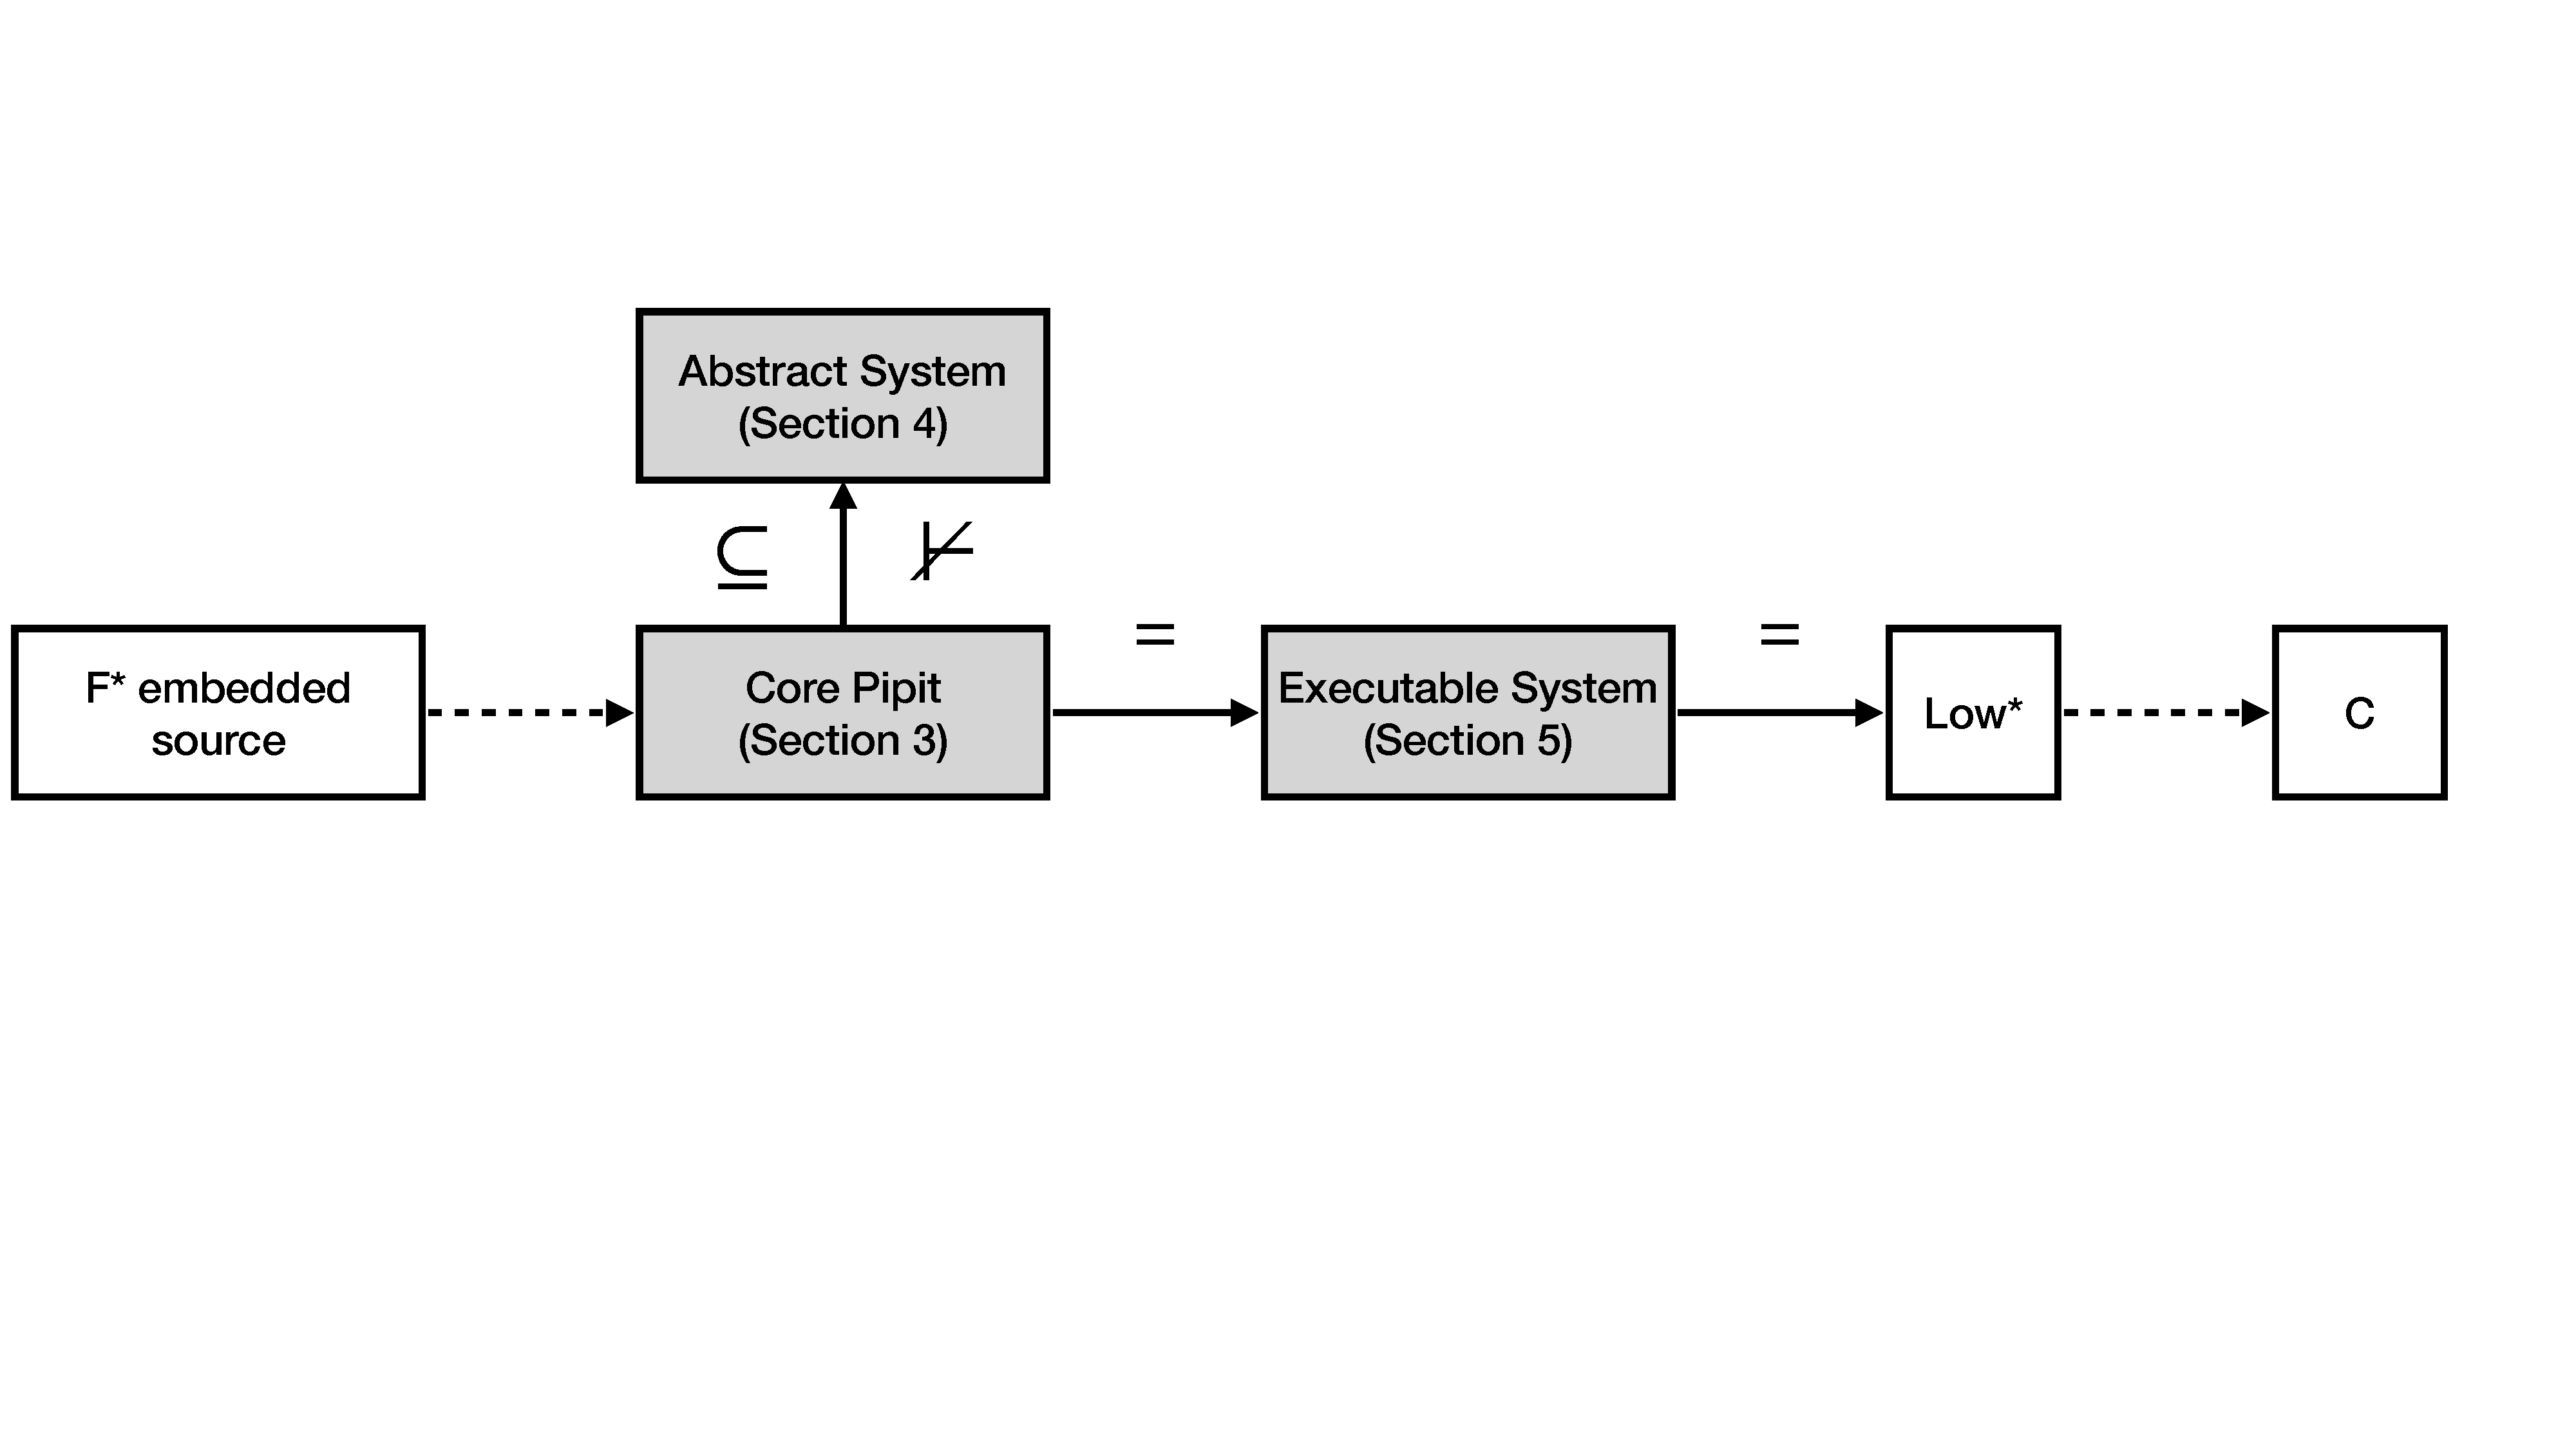
\includegraphics[width=\textwidth]{figures/core-structure.pdf}
\caption{Architecture of Pipit. The gray boxes and solid arrows are defined in this paper. The white boxes and dashed arrows are trusted components. The labels next to the arrows denote properties of the translation. The refinement label ($\subseteq$) indicates a verified abstraction relation; the negated entailment ($\not\vdash$) indicates that the entailment relation --- contracts and checked properties proven on abstract system apply to the checked semantics --- is not yet verified; the equivalence ($=$) denotes a verified equivalence relation.}
\label{f:core:structure}
\end{figure}
